\begin{problem}[14]
轴承问题中是否应该考虑惯性力的作用? 说明理由.
\end{problem}
% --------------------------------------------------------------------
\begin{solution}
\begin{minipage}[c]{0.8\linewidth}
如右图所示, 定承半径为$R$, 滑面平均间隙为$h$(轴的半径$r=R-h$), 润滑介质的粘性系数为$\mu$, 密度为$\rho$, 环境压力为$p_0$, 轴所担负的载重为$W$, 滑面相对速度$v$. 
在轴承润滑问题中, 存在三种力, 即惯性力, 粘性力和压力. 标志惯性力和粘性力之比为
\[
\frac{\text{惯性力}}{\text{粘性力}}=(\mathrm{Re})_h\cdot \frac{h}{R} < 10^{-3} \ll 1
\]
\end{minipage}
\begin{minipage}[c]{0.2\linewidth}
\begin{center}
\usetikzlibrary{calc,intersections,through,backgrounds}
\usetikzlibrary{decorations.pathreplacing,decorations.pathmorphing,arrows}
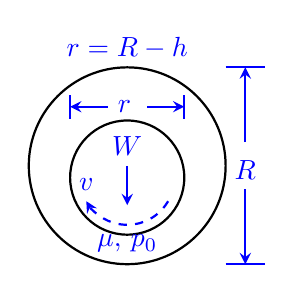
\begin{tikzpicture}
   \draw[thick] (0,0) circle(1.25) (0,-0.15) circle(0.725) node[below=17pt,blue]{$\mu$, $p_0$};
   \draw[thick,blue,->,>=stealth, dashed](0,-0.15)++(-30:0.6) arc(-30:-150:0.6) node[above] {$v$};
  \draw [thick,blue,->,>=stealth](0,0) node[above]{$W$}--(0,-0.5);
  \draw[thick,blue] (1.25,-1.25) -- (1.75,-1.25) (1.25,1.25) -- (1.75,1.25)
                                     (-0.725,0.6)--(-0.725,0.9) (0.725,0.6)--(0.725,0.9);

  \draw[thick,blue,<-,>=stealth] (1.5,-1.25)--(1.5,-0.3) node[above]{$R$};
  \draw[thick,blue,->,>=stealth](1.5,0.3)--(1.5,1.25);
 \node[blue] at (0,1.5){$r=R-h$};

  \draw[thick,blue,<-,>=stealth] (-0.725,0.75)--(-0.25,0.75) node[right]{$r$};
  \draw[thick,blue,<-,>=stealth] (0.725,0.75)--(0.25,0.75);
\end{tikzpicture}
\end{center}
\end{minipage}\vspace{5pt}
其中$(\mathrm{Re})_h=\rho v h/\mu$. 所以可忽略惯性力的影响.
\end{solution}
